\newpage
\section{Circuit Elements}

\subsection{Voltage and Current Sources}

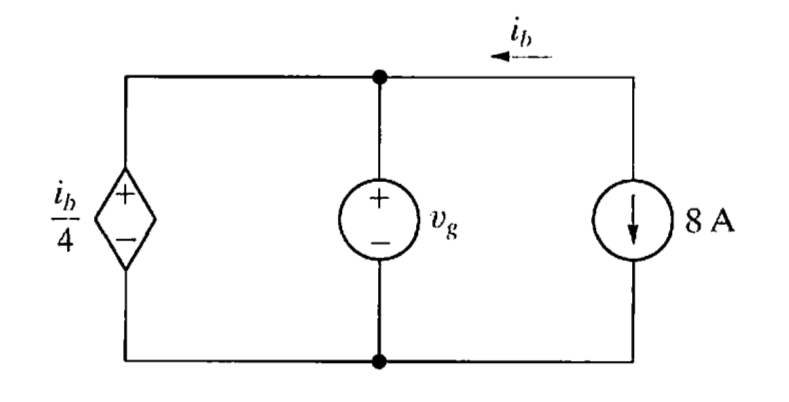
\includegraphics[scale=0.25]{img/c2/p1}
For the above circuit:
\begin{enumerate}
	\item What value of $v_g$ is required in order for the interconnection to be valid?
	\item For this value of $v_g$ find the power associated with the 8 A source.
\end{enumerate}

1) Notice that the current $i_b$ is in the same circuit branch as the 8 A source, but is defined
in the opposite direction. Therefore we can say that.
\\ \( i_b = -8\)A
\\Next, we can see that the dependent and independent voltage source are in parallel with the same
polarity. Therefore, we know that they must be equal. So if the dependent source is:

\begin{align*}
	V_{dependent} &= \frac{i_b}{4}
	\\ V_{dependent} &= V_g
	\\ V_g &= \frac{i_b}{4}
	\\ V_g &= \frac{-8}{4}
	\\ V_g &= -2V
\end{align*}

Therefore the answer to part 1 is -2 V. 


2) To find the power that corresponds to the 8 A source, we find the voltage drop across the source
which is $V_i$. This will also need to be equal to $V_g$. Therefore, $V_i$ will also equal -2 V.
Using passive sign convention we get:

\begin{align*}
	p_s &= (8 A)(V_i)
	\\ p_s &= (8 A)(-2 V)
	\\ p_s &= -16 W
\end{align*}

Therefore the current source generates 16 W of power. 

\newpage
\subsection{Ohm's Law}
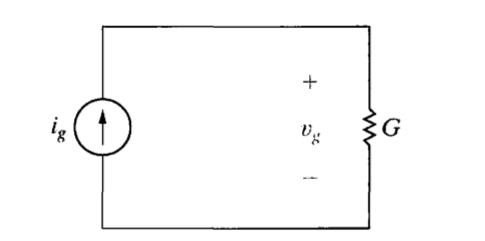
\includegraphics[scale=0.25]{img/c2/p2}

For the above circuit
\begin{enumerate}
	\item If $i_g = 0.5$ A and $G = 50$ mS, find $v_g$ and the power delivered by the current
	source
	\item If $v_g = 15$ V and the power delivered to the conductor is 9 W, find the conductance
	G and the source current $i_g$.
	\item If $G = 200 \mu S$ and the power delivered to the conductance is 8 W, find $i_g$ and 
	$v_g$
\end{enumerate}

1) You can see in the circuit that since G and $i_g$ are in the same branch, they must have
the same current. The voltage drop across the current source and G must also be equal, because
they are in parallel. Therefore, using Ohm's law we can solve for the voltage:

\begin{align*}
	V &= iR \\
	V &= \frac{i}{conductance} \\
	v_{g} &= \frac{i_g}{G} \\
	v_{g} &= \frac{0.5 A}{50mS} \\
	v_{g} &= 10 V
\end{align*}

Now we know the voltage we can solve for the power. 

\begin{align*}
	P &= Vi \\
	p_{source} &= -v_{i}i_{g} \\
	p_{source} &= -(10 V)(0.5 A) \\
	p_{source} &= -5 W	
\end{align*}

Thus the current source delivers 5 W to the circuit. 

2) First, we find the value of the conductance using the power and voltage. 

\begin{align*}	
	P &= VI \\
	V &= IR \\
	I &= \frac{V}{R} \\
	I &= V \times G \\
	P &= V^2 G \\
	p_{g} &= Gv_{g}^{2} \\
	G &= \frac{p_g}{v_{g}^{2}} \\
	G &= \frac{9}{15^{2}} \\
	G &= 0.04 S \\
	G &= 40 mS
\end{align*}

Then we can solve for the current:

\begin{align*}
	i_g &= G v_g \\
	i_g &= (40 mS)(15 V) \\
	i_g &= 0.6 A
\end{align*}


\newpage
\subsection{Kirchhoff's Law}
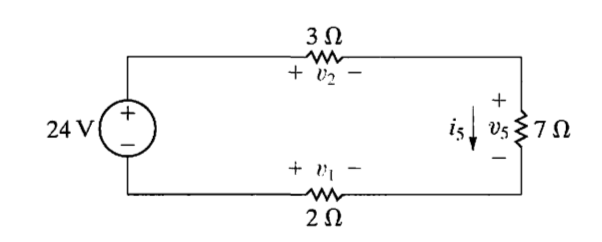
\includegraphics[scale=0.25]{img/c2/p3}

For the problem above, calculate:
\begin{enumerate}
	\item $i_5$
	\item $v_1$
	\item $v_2$
	\item $v_5$
	\item The power delivered by the 24 V source
\end{enumerate}


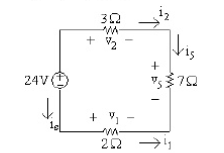
\includegraphics[scale=0.25]{img/c2/a3}
1) First redraw the circuit as shown above, adding in the new labels. Then, write a KVL equation
clockwise around the circuit. 
\\ \( -24 V + v_2 + v5 - v1 = 0 \)\\
Next, we can use Ohm's law to calculate the three unknown voltages. 

\begin{align*}
	v2 &= 3i_2 \\
	v5 &= 7i_5 \\
	v1 &= 2i_1 \\
\end{align*}

Using KCL in the upper right corner we can see that $i_2 = i_5$. In the bottom right corner we see
that $i_5 = -i_1$. In the upper left corner we can see that $i_s = -i_2$. We can then substitute
these into the previous three equations to get. 

\begin{align*}
	v2 &= 3i_2 = 3i_5 \\
	v5 &= 7i_5 \\
	v1 &= 2i_1 = -2i_5\\
\end{align*} 

Then we can substitute these equations into the first equation to get:
\begin{align*}
	24 &= v_2 + v_5 - v_1 \\
	24 &= 3i_5 + 7i_5 - (-2i_5) \\
	24 &= 12i_5 \\
	2 A &= i_5 \\
\end{align*}

We can then use this information to solve for the remaining variables. 
2) 
\begin{align*}
	v_1 &= -2i_5 \\
	v_1 &= -2(2) \\
	v_1 &= -4 V
\end{align*}

3)
\begin{align*}
	v_2 &= 3i_5 \\
	v_2 &= 3(2) \\
	v_2 &= 6 V \\
\end{align*}

4)
\begin{align*}
	v_5 &= 7i_5 \\
	v_5 &= 7(2) \\
	v_5 &= 14 V \\
\end{align*}

5) A KCL equation at the lower left node gives $i_s = i_1$ and since we know that $i_1 = -i_5$, then
$i_s = -2A$. Therefore:

\begin{align*}
	p_24 &= (24)i_s \\
	p_24 &= (24)(-2) \\
	p_24 &= -48 W
\end{align*}
 
So we can see the source is delivering 48 W. 

\newpage
\subsection{Analysis of Circuit Containing Dependent Sources}
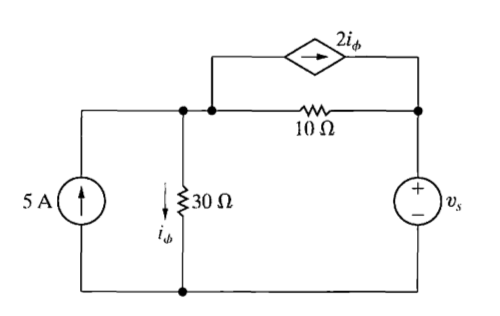
\includegraphics[scale=0.25]{img/c2/p4}

For the above circuit. The current $i_{\phi}$ is 2 A. Calculate:
\begin{enumerate}
	\item $v_s$
	\item The power absorbed by the independent voltage source,
	\item The power delivered by the independent current source,
	\item the power delivered by the controlled current source,
	\item the total power dissipated in the two resistors
\end{enumerate}

The problem tells us that $i_{\phi}$ is 2A, so we know that the current in the dependent source is $2i_{\phi} = 2(2) = 4A$ We can then write a KCL equation in the left node to find the current in the 
$10\Omega$ resistor.

\begin{align*}
	0 &= -5A + 2A +4A + i_{10\Omega} \\
	i_{10\Omega} &= 5A - 2A - 4A \\
	i_{10\Omega} &= -1 A
\end{align*}
We can then redraw the circuit as shown below. 
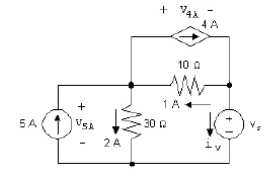
\includegraphics[scale=0.25]{img/c2/a4}

1) To find $v_s$, we can write a KVL equation that sums the voltages counter-clockwise around the 
lower right loop. 

\begin{align*}
	0 &= -v_s + (1A)(10 \Omega) + (2A)(30 \Omega) \\
	v_s &= 10V + 60V \\
	v_s &= 70 V
\end{align*}

2) The current in the voltage source can be found by writing a KCL equation at the right-hand node. 

\begin{align*}
	0 &= -4 A + 1 A + i_v \\
	i_v &= 4A - 1A \\
	i_v &= 3A 
\end{align*}

Therefore power is:
\begin{align*}
	p &= vi \\
	p &= (70 V)(3 A) \\
	p &= 210 W
\end{align*}

Thus the voltage source absorbs 210 W. 

3) The voltage drop across the independent current source can be found through a KVL equation around 
the left loop. 

\begin{align*}
	0 &= -v_{5a} + (2A)(30\Omega) \\
	v_{5a}	= &60 V \\
	p &= -v_{5a}i \\
	p &= -(60V)(5A) \\
	p &= -300 W \\
\end{align*}

Therefore the source delivers 300 W to the circuit. 

4) The voltage across the controlled current source can be found by writing a KVL equation
around the upper right loop in a clockwise direction:

\begin{align*}
	0 &= v_{4A} + (10\Omega)(1A) \\
	v_{4A} &= -10 V \\
	p &= v_{4A}i \\
	p &= (-10 V)(4 A) \\
	p &= -40 W
\end{align*}

Thus the source delivers 40 W of power to the circuit. 

5) The total power dissipated by the resistors is:

\begin{align*}
	&= (i_{30\Omega})^2(30\Omega) + (i_{10\Omega})^2(10\Omega) \\
	&= (2)^2(30\Omega)+(1)^2(10\Omega) \\
	&= 120 + 10 \\
	&= 130 W \\
\end{align*}


